\section {物料管理}

-

    \begin{center}
        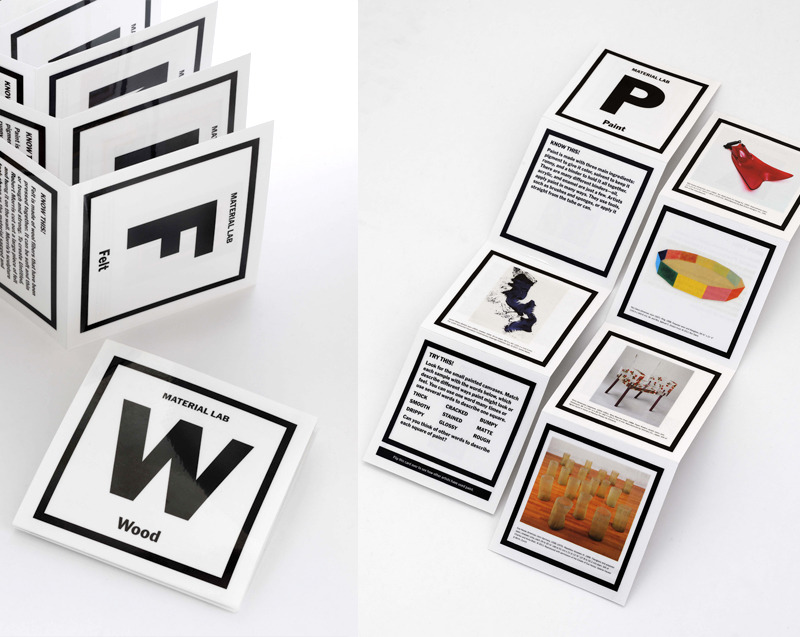
\includegraphics[scale=.3] {cards.jpg}
    \end{center}

    物料管理是将管理功能导入企业产销活动过程中,希望以经济有效的方法,及时取得供应组织内部所需之各种活动。

    物料管理概念的采用起源于第二次世界大战中航空工业出现的难题。生产飞机需要大量单个部件,很多部件都非常复杂,而且必须符合严格的质量标准,这些部件又从地域分布广泛的成千上万家供应商那里采购,很多部件对最终产品的整体功能至关重要。

    物料管理概念的采用起源于第二次世界大战中航空工业出现的难题。

    生产飞机需要大量单个部件,很多部件都非常复杂,而且必须符合严格的质量标准,这些部件又从地域分布广泛的成千上万家供应商那里采购,很多部件对最终产品的整体功能至关重要。物料管理就是从整个公司的角度来解决物料问题,包括协调不同供应商之间的协作,使不同物料之间的配合性和性能表现符合设计要求;提供不同供应商之间以及供应商与公司各部门之间交流的平台;控制物料流动率。计算机被引入企业后,更进一步为实行物料管理创造了有利条件,物料管理的作用发挥到了极致。

\subsection {物料的定义和特性}

    组成产品结构的最小单元是物料。在英文里“物料”有多种叫法,当我们说“物料需求计划” 时,“物料” 在英文里对应的是 materia1。 当我们说 “物料编码” 时,英文里的物料是 item 或 part。在一些国产 ERP 软件里,也有用 “物项”、 “物品”、 “物件”的,很不统一。我们顺着“物料需求计划”的词义,采用“物料”的叫法。

    这里所说的物料,指的是:凡是要列入计划、控制库存、控制成本的物件的统称。包括所有的原材料、配套件、毛坯、半成品、联产品、 副产品、回收品、需要处理的废品、包装材料、标签、说明书、技术文件、合格证、产成品、工艺装备、甚至可以是不能存储的某些能源等。换句话说,物料是计划的对象,库存的对象和成本的对象。

    从管理学角度看,物料的管理特性(家乡材料有物理性能和化学性能一样)主要是3个方面。

    \begin{enumerate}
        \item 相关性

        从供需链的概念出发,任何一种物料都是由于某种需求而存在的,没有需求的物料,就没有产生或保存的必要。一种物料的消耗量受另一种物料的需求量制约,如购买原材料是为了加工零件,而生产零件又是为了装配产品; MRP 理念的基本出发点就是平衡供需关系。从大范围来讲,一个企业的原料是另一个企业的产品= 一一个企业的产品,又是另一个企业的原料。

        只有当市场有需求时,企业生产的产品才有价值。这种相关需求不但有品种规格、性能、质量和数量的要求,而且有时间和空间 (需用时间和地点) 的要求。

        \item 流动性

        既然任何物料都是由于某种需要而存在,它就必然处于经常流动的状态,而不应当在某个地点长期滞留。物料的相关性必然形成物料的流动性,不流动的物料只能是一种没有需求的积压浪费。通过物料的流动性来检查物料在相关性上存在的问题,是物料管理或物流管理的一项重要内容。

        \item 价值

        物料是有价值的。库存或存货是流动资产,要占用资金; 而资金又是有时间价值的,使用了资金就应体现资金成本,要产生利润。因此,不仅要把库存物料看成是一种资产,还要看到它也是一种 "负债”(尤其是超储物料); 它占用了企业本来可以用来在其他方面获取利润的资金 应当计算机会成本。产品研发人员需要知道每个零部件的价值,从设计源头把住成本关,这也是价值工程学要做的分析工作。

    \end{enumerate}

    只有理解物料的这些管理特性 才能应用好 ERP 系统,做好计划管理、物料管理。

\subsection { 物料管理的目标}

    \begin{enumerate}
        \item  物料规格标准化,减少物料种类,有效管理物料规格的新增与变更。
        \item  适时供应生产所需之物料,避免停工待料。
        \item  适当管制采购价格,降低物料成本。
        \item  确保来料品质良好,并适当的管制供货商。
        \item  有效率的收发物料,提高工作人员之效率,避免呆料、废料之产生。
        \item  掌握物料适当的存量,减少资金的积压。
        \item  可考核物料管理之绩效。
        \item  仓储空间充分的利用。
    \end{enumerate}

\subsection { 物料的分类}

    \subsubsection {(一)功用}

    将材料分为主要材料与辅助材料。主要材料是构成制成品最主要之部份,而辅助材料多半在配合主要材料之加工而附属于制品上。

    \subsubsection {(二)型态}

    将材料分为素材与成型材。素材者仍需加工之材料,它又分为料材与粗型材。成型材为已加工之材料,它又分为配件、零件、组合件。

    \subsubsection {(三)成本管制}

    将材料分为直接材料与间接材料。直接材料使直接供作制品制造之材料,其消耗与产品之产量成正比,如铸件之于马达。间接材料是间接帮助制品之材料,其消耗不一定与产品之产量成正比,辅助材料有时亦包括于间接材料。

    \subsubsection {(四)调度方法}

    将材料分为公司外部调度的第一次材料与公司内部调度的第二次材料。公司外部调度的第一次材料系指公司内购、外购之材料与外加工之材料。第二次材料系指规模较大的公司内部部门很多,由一个部门之材料调度至另一部门。

    \subsubsection {(五)准备方法}

    将材料分为常备材料和非常常备材料。常备材料为利用存货管制的原理,定时购买一定数量的材料,存备这些材料以供生产之需。有些特殊材料不能事先购买存备,必须是生产计划而随时决定购买之材料,是为非常备材料。

\subsection { 物料的特性}

    首先是物料的相关性,任何物料总是由于有某种需求而存在;没有需求的物料就没有存在的必要。

    其次是物料的流动性,既然有需求,物料总是不断从供方向需方流动;物料的相关性决定了物料的流动性。

    物料是有价值的,一方面它占用资金,为了加速资金周转,就要加快物料流动;而另一方面,在物料形态变化和流动的过程中,要用创新竞争(不仅是削价竞争),提高物料的技术含量和附加值,用最小的成本、最短的周期、最优的服务,向客户提供最满意的价值并为企业自身带来相应的利润。这也是增值链(value-added chain)含义之所在。 三种特性相互作用、互相影响。理解物料的管理特性有助于理解物料需求管理的特点。

    在市场竞争日益激烈的环境下,产品生命周期越来越短,品种越来越多;客户对交货期的要求越来越短;同时,企业对库存的控制也因为成本的压力而变得越来越严格。怎样才能有效地解决这一矛盾,是摆在企业管理者面前的难题。本课程采集了大量不同行业和不同生产组织方式的企业物流模型,结合企业内部供应链管理研究的最新成果,理论结合实际,全方位演绎企业物流管理的真谛,帮助企业建立供应链管理的新模式。

\subsection { 物料管理的原则}

    通常意义上,物料管理部门应保证物料供应适时、适质、适量、适价、适地,这就是物料管理的5R原则,是对任何公司均适用且实用的原则,也易于理解和接受,下面分别进行阐述:

    \begin{enumerate}
    \item  适时:即要求供应商在规定的时间准时交货,防止交货延迟和提前交货。

    供应商交货延迟会增加成本,主要表现在:
        \begin{enumerate}
            \item  由于物料延迟,车间工序发生空等或耽搁,打击员工士气,导致效率降低、浪费生产时间;
            \item  为恢复正常生产计划,车间需要加班或在法定假期出勤,导致工时费用增加。
        \end{enumerate}

    因此应尽早发现有可能的交货延迟,从而防止其发生;同时也应该控制无理由的提前交货,提前交货同样会增加成本,主要原因为:
        \begin{enumerate}
            \item  交货提前造成库存加大,库存维持费用提高;
            \item  占用大量流动资金,导致公司资金运用效率恶化。
        \end{enumerate}

    \item  适质:即供应商送来的物料和仓库发到生产现场的物料,质量应是适当的,符合技术要求的。

    保证物料适质的方法如下:
        \begin{enumerate}
            \item  公司应与供应商签订质量保证协议;
            \item  设立来料检查职能,对物料的质量做确认和控制;
            \item  必要时,派检验人员驻供应商工厂(一般针对长期合作的稳定的供应商采用,且下给该供应商的订单达到其产能的30\%以上);同时不应将某个检验人员长期派往一个供应商处,以防其间关系发生变化;
            \item  必要时或定期对供应商质量体系进行审查;
            \item  定期对供应商进行评比,促进供应商之间形成良性有效的竞争机制;
            \item  对低价位、中低质量水平的供应商制订质量扶持计划;
            \item  必要时,邀请第三方权威机构做质量验证。
        \end{enumerate}

    \item  适量:采购物料的数量应是适当的,即对买方来说是经济的订货数量,对卖方而言为经济的受订数量。

    确定适当的订货数量应考虑以下因素:
        \begin{enumerate}
            \item  价格随采订货数量大小而变化的幅度,一般来说,订货数量越大,价格越低;
            \item  订货次数和采购费用;
            \item  库存维持费用和库存投资的利息。
        \end{enumerate}

    \item  适价:采购价格的高低直接关系到最终产品或服务价格的高低,在确保满足其它条件的情况下力争最低的采购价格是采购人员最重要的工作。

    采购部门的职能包括标准化组件,发展供应商,发展替代用品,评估和分析供应商的行为。为了达到这一目标,采购部门应该在以下领域拥有决策权:
        \begin{enumerate}
            \item  选择和确定供应商;
            \item  使用任何一种合适的定价方法;
            \item  对物料提出替代品;

            采购部门通常能够提供出目前在用物料的替代品,而且它也有责任提请使用者和申请采购者关注这些替代品。当然,是否接受这些替代品要由使用者/设计人员最终作出决定;
            \item  与潜在的供应商保持联系。

            采购部门必须和潜在的供应商保持联系。如果使用者直接与供应商联系,而采购部门又对此一无所知的话,将会产生“后门销售”,即潜在的供应商通过影响使用者对物料规格方面的要求成为唯一的供应商,或是申请采购者私下给供应商一些许诺,从而使采购部门不能以最低的价格签订理想的合同。如果供应商的技术人员需要和公司技术人员或生产人员直接交换意见,采购部门应该负责安排会谈并对谈判结果进行审核。
        \end{enumerate}

    \item  适地:物料原产地的地点应适当,与使用地的距离越近越好。距离太远,运输成本大,无疑会影响价格,同时沟通协调、处理问题很不方便,容易造成交货延迟。

    高科技行业对产品质量普遍要求很高,致使各企业对生产制造环节管理越来越精细,但对产品的物料管理环节却依旧保持比较粗放的管理风格,使物料在很大程度上占用了企业资金,无形中导致成本增长,利润下降。物料管理是企业内部物流各个环节的交叉点,衔接采购与生产、生产与销售等重要环节,关乎企业成本与利润的生命线,不仅如此,物料管理还是物资流转的重要枢纽,甚至关系到一个企业存亡。曾听过一个关于爱多的例子,据说爱多在破产之际,库存物料的金额高达上亿元,可就是这么多的物料中,居然无法组装出一个完整的DVD成品,在惊叹之余,更激起人们对于制造企业物料呆滞及不合理管库问题的思考。

    有资料表明,企业的存货资金平均占用流动资产总额的40\%-50\%,而高科技制造企业的库存比例则远高于此。“物料存在两套或多套编码”、“物料混乱堆积在仓库各个角落”,成为许多制造企业仓库的真实写照。就曾有人套用中央电视台著名的广告语“心有多大,舞台就有多大”放在制造型企业身上,演绎成“仓库有多大,库存就有多高”,形象地表述了普遍存在于制造型企业内部库存管理问题的顽疾。

    \end{enumerate}

\subsection { 物料管理的职能机构}

    一个小公司的发展可分为三个阶段:完全整合、职能独立、相关职能的再整合。

    一个公司初创时,几乎所有的工作都是由总经理(通常是公司的所有者)或是组成领导小组的公司主要成员来完成的。

    随着公司的发展和壮大,公司业务量和工作人员逐渐增多,相应的职能逐步独立形成职能部门,例如,采购、仓储、运输、生产计划、库存控制和质量控制等职能都形成了独立的部门,并致力于专门的管理工作,公司业务上的分工也日益专业化。

    各职能部门独立后,各部门之间的沟通机会越来越少,于是部门之间合作的问题经常出现,矛盾一点点加深。最终我们又可以清楚地看到,如果能减少由于沟通和合作而产生的问题,把相互之间有密切联系的职能部门重新加以整合,公司就可以极大程度地受益。

    于是,与物料管理有密切联系的各职能部门被重新整合到一起。

\subsubsection {部门的职能范围}

    一般来说,物料管理部门的职能包括以下方面:

    \begin{itemize}
    \item  物料的计划和控制

        即根据项目主合同交货时间表、车间生产计划和项目技术文件等确定物料需求计划,并根据实际情况和项目技术更改通知等文件随时调整物料需求数量,控制项目材料采购进度和采购数量。

    \item  生产计划

        根据项目主合同交货时间表和材料采购进度编制车间生产计划,并根据实际情况和项目计划随时调整,使车间生产计划与项目主合同交货时间表保持一致。

    \item  采购

    根据车间生产计划对生产所需要的物料进行准确的分析,并制订完整的采购计划;严格地控制供应商的交货期和交货数量;

    \item  物料和采购的研究

        收集、分类和分析必要的数据以寻找替代材料;对主要外购材料的价格趋势进行预测;对供应商成本和能力进行分析;开发新的、更为有效的数据处理方法,从而使物料系统更加高效地运转。

    \item  来料质量控制

        即对供应商的交货及时进行来料检查,及时发现来料的质量问题以便于供应商有足够时间处理或补发产品,保证车间及时得到物料供应,保证发送到车间现场的物料全部是合格产品。

    \item  物料收发

        负责物料的实际接收处理、验明、通知质量作来料质量检验,以及将物料向使用地点和仓储地点发送。

    \item  仓储

        对接收入库的物料以正确的方式进行保管、储存,对储存过程中可能变质或腐蚀的物料,应按一定的防腐蚀和变质的方法进行清洗、防护、特殊包装和存放。

    \item  库存控制

        定期检查物料库存状况,加强物料进出库管理;随时掌握库存变化情况,发现任何异常(包括呆滞料,库存积压或0库存)情况,及时向采购通报。

    \end{itemize}

    当然,并不是所有公司的物料管理部门都包括上述所有职能。根据公司规模大小,公司业务性质不同以及公司不同发展阶段,物料管理部门的职能也不尽相同。

    通过上述文字描述,可知与物料有密切联系的各职能部门被重新整合到一起,这种整合就是物料管理理论的基础,所以,物料管理较仓库管理的范围更为广泛,其中也包括仓库管理。
